\begin{quote}
    \textit{``I could draw here AdS, but I know most of you here are allergic to that.'' --Jorge Santos}
\end{quote}

Today, we will introduce the initial value problem in general relativity. In classical physics, it's natural to say that we set initial conditions and (using some differential equations) evolve them to the future. But in GR, the question is more complicated because we are trying to evolve things to ``the future,'' yet the future is part of what we are solving for! It will take some care to define precisely what we mean.

\begin{defn}
    Let $(\cM,g)$ be a time-orientable spacetime. A \term{partial Cauchy surface} $\Sigma$ is a hypersurface for which no two points $p,p'\in \Sigma$ are connected by a causal curve in $\cM$.
\end{defn}
\begin{defn}
    The \term{future domain of dependence} of $\Sigma$, denoted $D^+(\Sigma)$, is the set $p\in \cM$ such that every past-inextendible causal curve through $p$ intersects $\Sigma$. The past domain of dependence $D^-(\Sigma)$ is defined equivalently for future-inextendible causal curves, and the domain of dependence is then $D(\Sigma)=D^+(\Sigma)\cup D^-(\Sigma)$.
\end{defn}
\begin{exm}
    Consider Minkowski space, with a partial Cauchy surface $\Sigma:t=0,x >0$. Then the domain of dependence $D(\Sigma)$ is the 45-degrees region with $x\geq |t|$-- see Fig. \ref{fig:domainofdependence} for an illustration.
\end{exm}

\begin{figure}
    \centering
    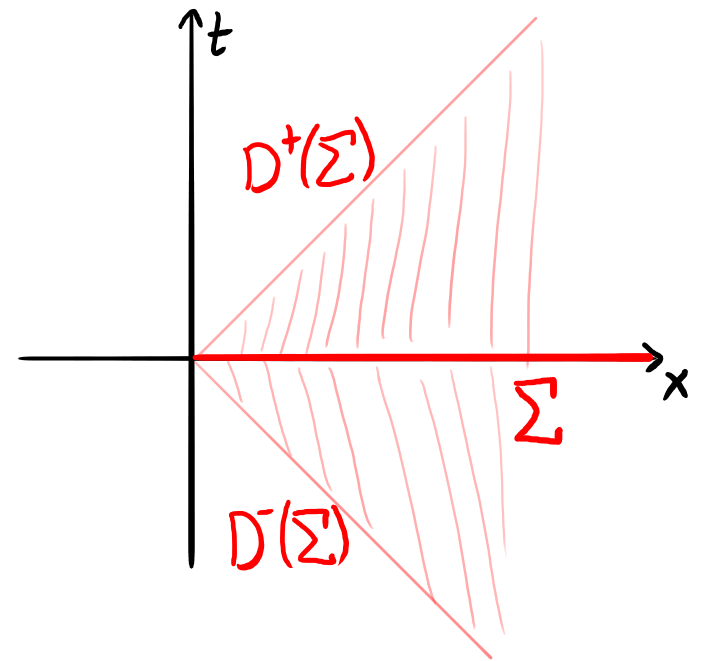
\includegraphics[width=0.5\textwidth]{2019/01/20190130_domainofdependence.png}
    \caption{In Minkowski space, we select the partial Cauchy surface $\Sigma:t=0,x>0$ (in red). Given initial conditions on $\Sigma$, we can predict physics in the shaded region $D^+(\Sigma)$ and retrodict in the region $D^-(\Sigma)$. However, $\Sigma$ is not a Cauchy surface because there are points in spacetime which lie outside the domain of dependence $D(\Sigma)$. Note also that the boundary of $D^+(\Sigma)$ (i.e. the Cauchy horizon) coincides with the boundary of the causal future of points outside $\Sigma$.}
    \label{fig:domainofdependence}
\end{figure}
\begin{defn}
    As far as we (as physicists) are concerned, a \term{hyperbolic partial differential equation} (second order) is defined to be a differential equation of the form
    \begin{equation}
        g^{ef} \nabla_e \nabla_f T^{ab\ldots}{}_{cd\ldots} = \tilde G^{ab\ldots}{}_{cd},
    \end{equation}
    where the tensor we've put on the RHS depends only on $T$ and first derivatives of $T$ in some smooth way. That is, the second derivative is the highest derivative, and it appears only linearly. These are sometimes called quasilinear equations.
\end{defn}
\begin{defn}
    A \term{Cauchy surface} for a spacetime $(\cM,g)$ is a partial Cauchy surface $\Sigma$ with $D(\Sigma)=\cM$ the entire manifold. Spacetimes $(\cM,g)$ which admit Cauchy surfaces are called \term{globally hyperbolic}.
\end{defn}
Note that if $D(\Sigma)\neq \cM$, then the solution of hyperbolic equations will \emph{not} be uniquely specified on $\cM\setminus D(\Sigma)$ by data on $\Sigma$.
%I could draw here AdS, but I know most of you here are allergic to that.
\begin{exm}
    A very simple example of a spacetime that is not globally hyperbolic is $\RR^{1,1}\setminus{0}$. There are points where a past-directed inextendible causal curve can drop off the manifold (i.e. hit the point we have removed).
\end{exm}
\begin{thm}[Wald]
    Let $(\cM,g)$ be a globally hyperbolic spacetime. Then
    \begin{enumerate}
        \item[(i)] There exists a global-time function $t:\cM \to \RR$ such that $-(dt)^a$ (the normal to surfaces of constant $t$) is future-directed and timelike.
        \item[(ii)] Surfaces of constant $t$, $\Sigma_t$, are Cauchy surfaces and all have the same topology.
        \item[(iii)] The topology of $\cM$ is $\RR\times \Sigma$.
    \end{enumerate}
\end{thm}
Remark: spacetimes which have singularities can still be globally hyperbolic. Consider the Kruskal spacetime-- we can set initial conditions on the Cauchy surface $U+V={}$constant.

\subsection*{Extrinsic curvature}
Let $\Sigma$ denote a spacelike or timelike hypersurface with unit normal $n_a$ (i.e. such that $n^a n_a=\pm 1$). We can define a projector onto this hypersurface $h^a{}_b$, which has some nice properties.
\begin{lem}
    For any $p\in \Sigma$, let $h^a{}_b = \delta^a{}_b \mp n^a n_b$ so that $h^a{}_b n^b =0$ (where upper/lower signs apply for spacelike/timelike respectively). Then
    \begin{enumerate}
        \item $h^a{}_c h^c{}_b=h^a{}_b$
        \item Any vector $x^a$ at $p$ can be written as $x^a_\parallel + x^a_\bot$, where $x^a_\parallel = h^a{}_b x^b$ and $x^a_\bot = \pm n_b x^b n^a$.
        \item If $X^a,Y^a$ are tangent to $\Sigma$, then $h^{ab} X_a Y_b=g^{ab} X_a Y_b$. $h$ is sometimes called the first fundamental form. 
    \end{enumerate}
\end{lem}
That is, let $N^a$ be normal to $\Sigma$ at a point $p$. If we parallel transport $N^a$ on $\Sigma$ along $X^a$ (i.e., obeying the equation $X^b \nabla_b N^a=0$), will the parallel-transported $N^a$ still be normal? Take $Y$ tangent to $\Sigma$, so that $Y^a N_a=0$ at the point $p$. Then
\begin{equation}
    \nabla_X (Y^a N_a)=X^b \nabla_b(Y^a N_a)=N_a X^b \nabla_b Y^a.
\end{equation}
\begin{defn}
    Up to now, $n_a$ has been defined only on $\Sigma$. First, let us extend it to a neighborhood of $\Sigma$ in an arbitrary way. The \term{extrinsic curvature} (second fundamental form) is defined at $p\in \Sigma$ by
    \begin{equation}
        K(X,Y)=-n_a(\nabla_{X_\parallel} Y_{\parallel})^a.
    \end{equation}
\end{defn}
Here, $X$ and $Y$ need not be tangent to $\Sigma$, but we are interested in their projections onto $\Sigma$. $K$ therefore represents the extent to which normal vectors on $\Sigma$ parallel-transported by vectors tangent to $\Sigma$ fail to be normal after parallel transport. In addition, $K$ does not look manifestly symmetric in $X$ and $Y$ written in this form, but in fact it is.

\begin{lem}
    $K_{ab}$ is independent of how $n_a$ is extended off $\Sigma$, and in particular
    \begin{equation}
        K_{ab}=h_a{}^c h_b{}^d \nabla_c n_d.
    \end{equation}
\end{lem}
\begin{proof}
    The RHS of $K(X,Y)$ is
    \begin{equation}
        -n_d X_\parallel^c \nabla_c Y^d_{\parallel} = X_\parallel^c Y^d \nabla_c n_d
    \end{equation}
    by the Leibniz rule, since $n_d Y^d_\parallel=0$. So
    \begin{equation}
        K(X,Y)=X_\parallel^c Y^d_\parallel \nabla_c n_d = X^a Y^b h_a{}^c h_b{}^d \nabla_c n_d.
    \end{equation}
    Therefore
    \begin{equation}
        K_{ab}=h_a{}^c h_b{}^d \nabla_c n_d.
    \end{equation}
    To demonstrate that $K_{ab}$ is independent of how $n_a$ is extended, consider a different extension $n_a'$, and let $m_a \equiv n_a'-n_a$. Note that on $\Sigma, m_a=0$. Then on $\Sigma$,
    \begin{align*}
        X^a Y^b(K'_{ab}-K_{ab}) &= X_\parallel^c Y^d_\parallel \nabla_c m_d\\
        &= \nabla_{x_\parallel}(Y_\parallel^d m_d)=0
    \end{align*}
    since $Y_\parallel^d m_d =0$ on $\Sigma$.
\end{proof}

We can use
\begin{equation}
    n^b \nabla_c n_b = \frac{1}{2} \nabla_c(n_b n^b)=0
\end{equation}
and conclude that
\begin{equation}
    K_{ab}=h_a{}^c \nabla_c n_b.
\end{equation}
At home, we should show that the extrinsic curvature is given by a Lie derivative,
\begin{equation}
    K_{ab}=\frac{1}{2} \cL_n (h_{ab})
\end{equation}
where $h$ here is the first fundamental form.

\subsection*{Non-lectured aside: extrinsic curvature is Lie derivative}

We want to show that
\begin{equation}
    K_{ab}=\frac{1}{2} \cL_n (h_{ab}).
\end{equation}
Let us compute the left side of this expression first:
\begin{equation}
    K_{ab}= h_a{}^c \nabla_c n_b = (\delta_a^c + n_a n^c) \delta_c n_d = n_a n_b + n_a n^c \nabla_c n_b.
\end{equation}
Note that by a lemma we'll prove in the next lecture, $K_{ab}$ is symmetric, so
\begin{equation}\label{expandedkab}
    K_{ab}= K_{(ab)}= \frac{1}{2}\paren{\nabla_a n_b + \nabla_b n_a + n_a n^c \nabla_c n_b + n_b n^c \nabla_c n_a}.
\end{equation}
Now the right side of the equality is
\begin{equation}
    (\cL_n h)_{\mu\nu} = n^\rho \p_\rho h_{\mu\nu} + h_{\mu\rho} \p_\nu n^\rho +h_{\rho \nu} \p_\mu n^\rho
\end{equation}
and promoting to covariant derivatives, we have
\begin{align}
    (\cL_n h)_{ab} &= n^c \nabla_c h_{ab} + h_{ac} \nabla_b n^c +h_{c b} \nabla_a n^c \nonumber\\
        &= n^c \nabla_c (g_{ab} + n_a n_b) + (g_{ac} +n_a n_c) \nabla_b n^c +(g_{cb}+n_c n_b) \nabla_a n^c \nonumber\\
        &= n_a n^c \nabla_c n_b + n_b n^c \nabla_c n_a + \nabla_b n_a + \nabla_a n_b,
\end{align}
where we have used metric compatibility and the property that $n_c \nabla_b n^c=0$. By comparison to Eqn. \ref{expandedkab}, we see that
\begin{equation*}
    K_{ab}=\frac{1}{2} (\cL_n h)_{ab}.
\end{equation*}
\qed